\chapter{Architektur}

\section{Architektur-Übersicht}
	Das folgende Diagramm zeigt eine Übersicht über die notwendigen Komponenten für eine Videoplattform mit JavaScript. Die Applikation ist als "`Fat-Client"'-Architektur aufgebaut. Es gibt keine Serverkomponenten für die Applikation selbst. Erst für den Verbindungsaufbau werden Vermittlungsserver benötigt.
	\begin{figure}[H]
		\centering
		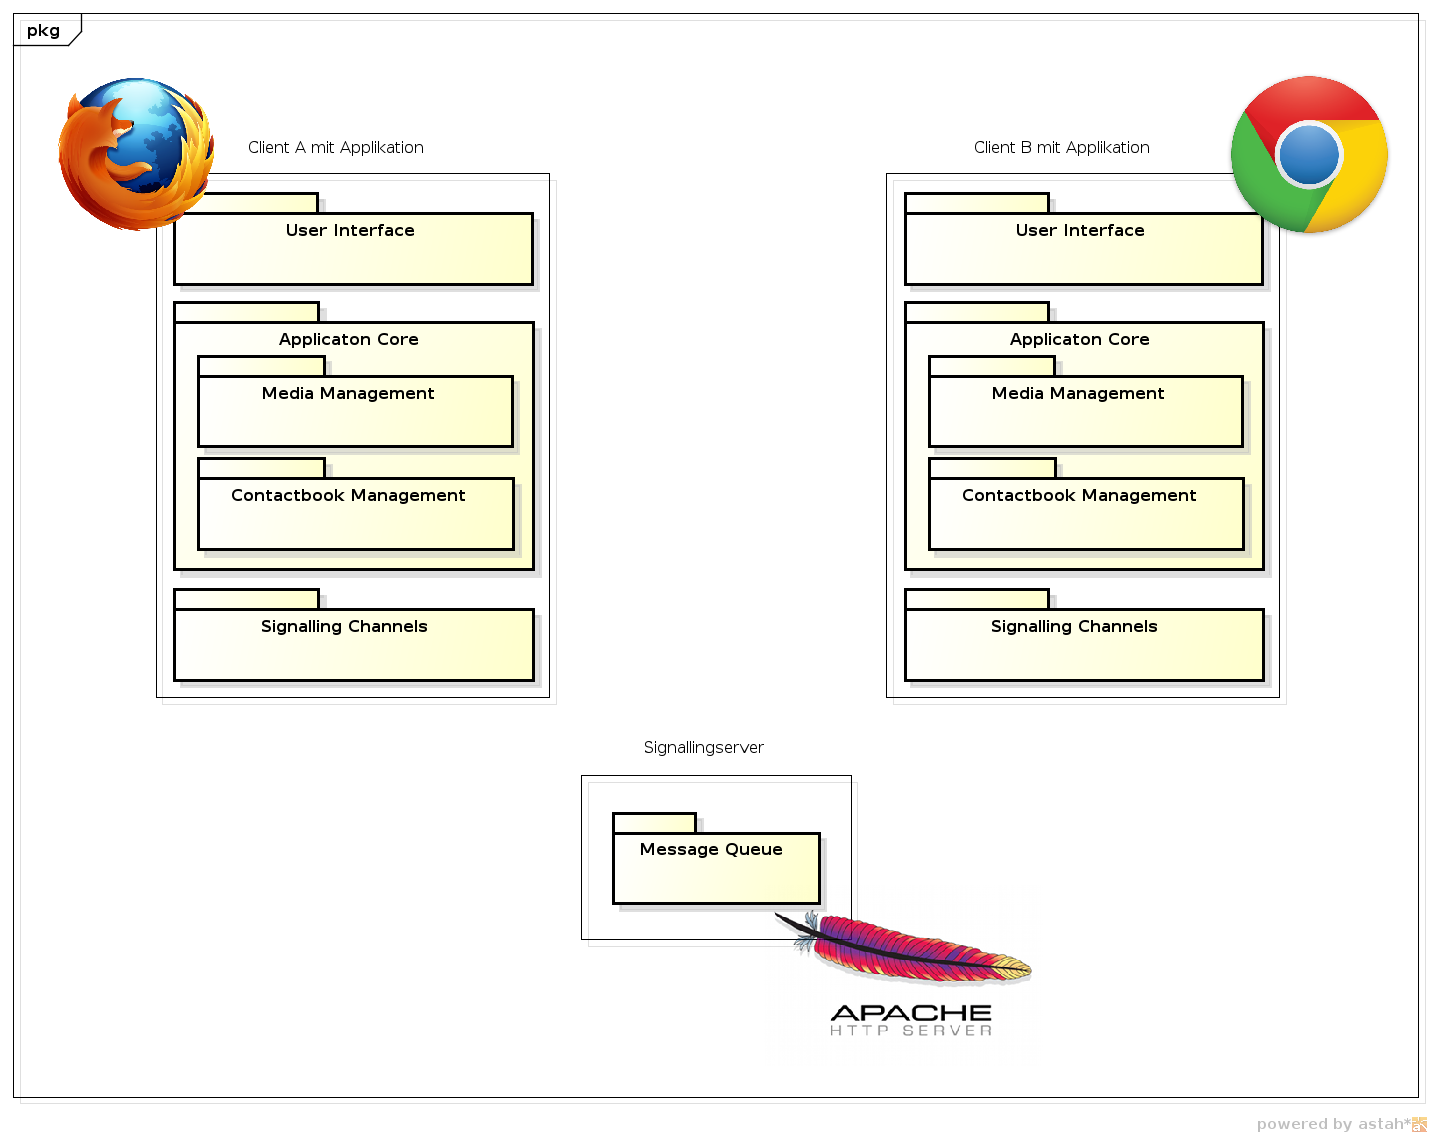
\includegraphics[width=1\textwidth]{../architekturanalayse/img/bigPicture.png}
		\caption{Big Picture JS VoIP App}
	\end{figure}
	
	Jeder Client besitzt Signaling Channels, die mit einem Signaling Server interagieren. Hier wurde als Beispiel eine Message Queue und ein SIP Server verwendet. Die Kommunikation läuft entsprechend über XHR oder SIP.
		
	Ein Verbindungsaufbau beginnt bei einem Client. Der Browser generiert eine Offer für den andern Client und sendet diese in einer Signaling Message über einen Signaling Server wie eine einfache Message Queue oder einen SIP Server an den andern Client. Der Browser des andern Clients generiert eine Answer und schickt diese auf dem gleichen Weg zurück. Anschliessend bauen die Clients die direkte P2P Connection auf. Sobald diese aufgebaut wurde, können Daten oder Video- und Audio gestreamt werden.
	
	Für den Abbau sendet ein Client ein bye. Anschliessend bauen beide Clients die P2P Connection ab.
	
	
	\subsection{Client/Server vs. reine Client-Applikation}
		\subsubsection{Vorteile Client/Server-Umsetzung}
		\begin{itemize}
			\item Schlanker Client
			\item Es wird nur eine Schnittstelle benötigt zwischen Client und Server, der gesamte Verkehr kann über HTTP abgewickelt werden.
			\item Nur der Server muss die Schnittstellen zu anderen Diensten
			unterstützen. Keine zusätzlichen Schnittstellen-Anforderungen an den Client.
			\item Es ist einfacher durch Firewalls durchzukommen, da die Kommunikation genau kontrolliert werden kann.
		\end{itemize}
		\subsubsection{Nachteile}
		\begin{itemize}
			\item Redundanzen, da Funktionalität zwischen Client und Server durch
			ein eigenes Protokoll abgebildet und damit auf beiden Seiten Teile derselben
			Funktionalität umgesetzt werden müssen.
			\item Ein Anwender ist an den Server oder die Serverimplementation gebunden.
			Die Applikation läuft nicht ohne den Server.
			\item Der Server ist ein "`Single Point of Failure"', falls keine redundanten Server eingesetzt werden. Zudem stellt der Server eine zentrale Angriffsstelle dar, über die Angreifer einfacher das ganze System blockieren könnten.
			\item Möchte ein Entwickler die Applikation um weitere Schnittstellen erweitern, so muss er Server und möglichweise den Client trotzdem auch anpassen, was aufwendiger ist. Zudem muss er den Server selbst betreiben und kann keinen bestehenden mehr nehmen was für Ihn zusätzlichen Aufwand bedeutet.
		\end{itemize}


		\subsubsection{Vorteile reine Client-Lösung}
		\begin{itemize}
			\item Es wird kein Server benötigt.
			\item Anwender können einen beliebigen Kommunikationsserver
			(beispielsweise SIP\footnote{Session Initiation Protocol \cite{IETF-SDP-RFC}} oder
			XMPP\footnote{Extensible Messaging and Presence Protocol}) für das
			Signaling verwenden und sogar selbst eine eigene Channelimplementation
			hinzufügen.
			\item Um die Applikation für weitere Schnittstellen zu erweitern sind keine
			Kenntnisse der Servertechnologie notwendig.
			\item Die Applikation ist insgesamt weniger aufwändig aufgebaut, da sie
			weniger Redundanzen beinhaltet.
			\item Es ist keine eigene SIP-/XMPP-Server-Implementation erforderlich
			(bereits vorhandene Serverinfrastrukturen werden genutzt).
		\end{itemize}
		\subsubsection{Nachteile}
		\begin{itemize}
			\item Die möglichen Schnittstellen sind auf die Browserfunktionalität
			begrenzt (HTTP, WebSockets, SDP, STUN, UserMedia). Dadurch
			muss ein SIP- oder XMPP-Provider WebSockets unterstützen, damit er für das
			Signaling genutzt werden kann.
			\item Der Client wird umfangreicher.
			\item Probleme mit Firewalls und Routern möglich, die WebSocket-Pakete nicht
			weiterleiten. WebSockets können grundsätzlich über einen beliebigen Port laufen, meist wird jedoch Port 80 verwendet.
			\item Performanceprobleme möglich, da sämtliche Logik, inklusive dem Parsen
			der verschiedenen Protokolle, vom Client abgearbeitet werden muss.
		\end{itemize}

		\subsubsection{Fazit}
			Aufgrund geringerer Abhängigkeiten und der Wahrscheinlichkeit, das die
			SIP-Server-Provider irgendwann WebSockets unterstützen, wird die Lösung
			"`reine Client Applikation"' gewählt.
			Für die Kommunikation mit Signalingservern, wie SIP oder XMPP, werden
			WebSockets eingesetzt, für das Signaling über XHR\footnote{XmlHTTPRequest}
			wird mit der Option "`Allow Cross Origin"' gearbeitet.

\section{Architektur-Schichten}
	Der logische Aufbau der Software besteht aus vier Schichten:
	\begin{figure}[H]
		\centering
		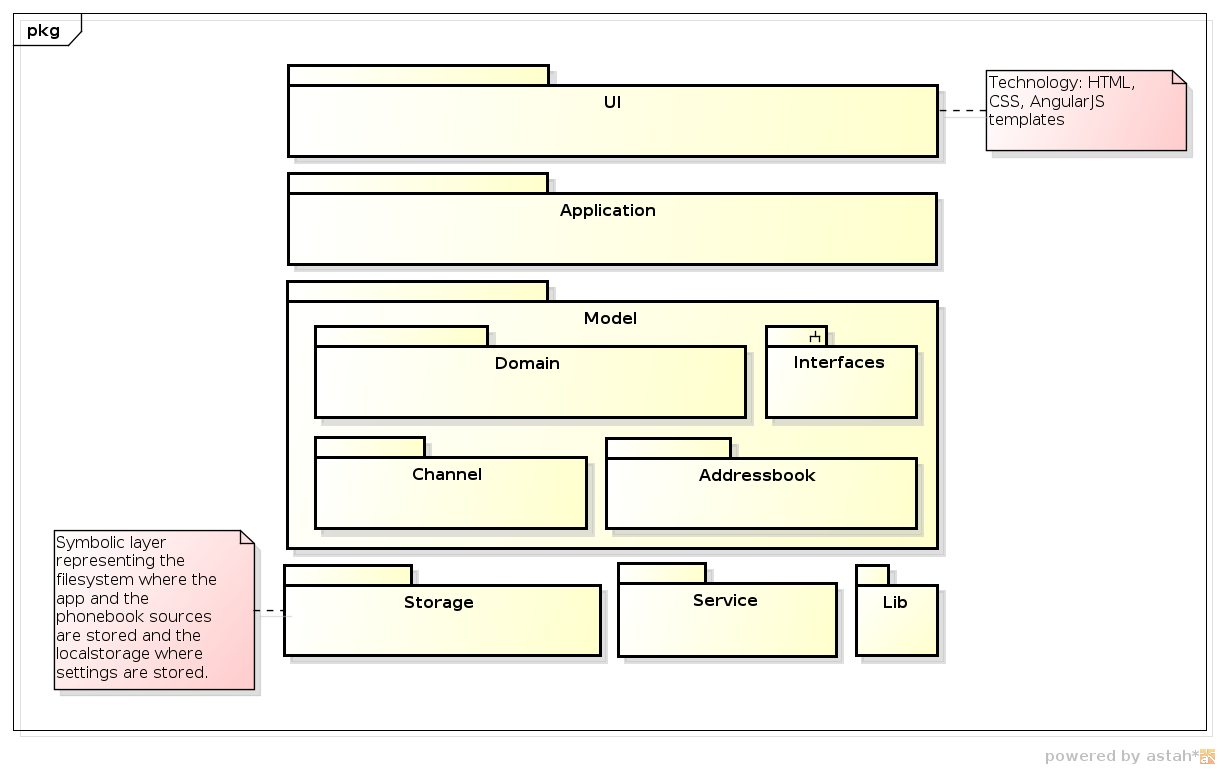
\includegraphics[width=1\textwidth]{../architekturanalayse/img/architecture.png}
		\caption{Architekturdiagramm JS VoIP App}
	\end{figure}
	Im untersten Layer sind Services und Libraries enthalten, auf die die oberen Layer zugreifen.
	Der Application Layer beinhaltet View Models für das User Interface und interagiert mit dem Model. 

